\documentclass[journal]{IEEEtran}
\usepackage{mdframed}
\usepackage{longtable} %for long tables to be fitted on multiple pages
\usepackage{ragged2e}
%\usepackage{color}
\usepackage{graphicx}
\usepackage{varioref}
\usepackage{epsfig}
\usepackage{times}
\usepackage[section]{placeins} % to keep floats(figures) in the section in which they were issued
\usepackage{amsmath}
\usepackage{amssymb}
\usepackage{url}
\usepackage{multirow}
\usepackage[T1]{fontenc}
\usepackage{ascii}
\usepackage{nomencl}
\usepackage{lscape}
\usepackage{longtable,tabu}
\usepackage{lmodern}
\usepackage{lipsum}
\usepackage[tight,footnotesize]{subfigure}
\usepackage{cite}
\usepackage[acronym]{glossaries} 
\usepackage{fancybox}
\usepackage{algorithmic}
\usepackage[boxed]{algorithm}
\usepackage[compact]{titlesec}

%----------For code listing---------------------------------------------------
\usepackage{listings} % Required for inserting code snippets
\graphicspath{{./}{images/}}
%% bare_jrnl.tex
%% V1.4b
%% 2015/08/26
%% by Michael Shell
%% see http://www.michaelshell.org/
%% for current contact information.
%%
%% This is a skeleton file demonstrating the use of IEEEtran.cls
%% (requires IEEEtran.cls version 1.8b or later) with an IEEE
%% journal paper.
%%
%% Support sites:
%% http://www.michaelshell.org/tex/ieeetran/
%% http://www.ctan.org/pkg/ieeetran
%% and
%% http://www.ieee.org/

%%*************************************************************************
%% Legal Notice:
%% This code is offered as-is without any warranty either expressed or
%% implied; without even the implied warranty of MERCHANTABILITY or
%% FITNESS FOR A PARTICULAR PURPOSE! 
%% User assumes all risk.
%% In no event shall the IEEE or any contributor to this code be liable for
%% any damages or losses, including, but not limited to, incidental,
%% consequential, or any other damages, resulting from the use or misuse
%% of any information contained here.
%%
%% All comments are the opinions of their respective authors and are not
%% necessarily endorsed by the IEEE.
%%
%% This work is distributed under the LaTeX Project Public License (LPPL)
%% ( http://www.latex-project.org/ ) version 1.3, and may be freely used,
%% distributed and modified. A copy of the LPPL, version 1.3, is included
%% in the base LaTeX documentation of all distributions of LaTeX released
%% 2003/12/01 or later.
%% Retain all contribution notices and credits.
%% ** Modified files should be clearly indicated as such, including  **
%% ** renaming them and changing author support contact information. **
%%*************************************************************************


% *** Authors should verify (and, if needed, correct) their LaTeX system  ***
% *** with the testflow diagnostic prior to trusting their LaTeX platform ***
% *** with production work. The IEEE's font choices and paper sizes can   ***
% *** trigger bugs that do not appear when using other class files.       ***                          ***
% The testflow support page is at:
% http://www.michaelshell.org/tex/testflow/




%
% If IEEEtran.cls has not been installed into the LaTeX system files,
% manually specify the path to it like:
% \documentclass[journal]{../sty/IEEEtran}





% Some very useful LaTeX packages include:
% (uncomment the ones you want to load)


% *** MISC UTILITY PACKAGES ***
%
%\usepackage{ifpdf}
% Heiko Oberdiek's ifpdf.sty is very useful if you need conditional
% compilation based on whether the output is pdf or dvi.
% usage:
% \ifpdf
%   % pdf code
% \else
%   % dvi code
% \fi
% The latest version of ifpdf.sty can be obtained from:
% http://www.ctan.org/pkg/ifpdf
% Also, note that IEEEtran.cls V1.7 and later provides a builtin
% \ifCLASSINFOpdf conditional that works the same way.
% When switching from latex to pdflatex and vice-versa, the compiler may
% have to be run twice to clear warning/error messages.






% *** CITATION PACKAGES ***
%
%\usepackage{cite}
% cite.sty was written by Donald Arseneau
% V1.6 and later of IEEEtran pre-defines the format of the cite.sty package
% \cite{} output to follow that of the IEEE. Loading the cite package will
% result in citation numbers being automatically sorted and properly
% "compressed/ranged". e.g., [1], [9], [2], [7], [5], [6] without using
% cite.sty will become [1], [2], [5]--[7], [9] using cite.sty. cite.sty's
% \cite will automatically add leading space, if needed. Use cite.sty's
% noadjust option (cite.sty V3.8 and later) if you want to turn this off
% such as if a citation ever needs to be enclosed in parenthesis.
% cite.sty is already installed on most LaTeX systems. Be sure and use
% version 5.0 (2009-03-20) and later if using hyperref.sty.
% The latest version can be obtained at:
% http://www.ctan.org/pkg/cite
% The documentation is contained in the cite.sty file itself.






% *** GRAPHICS RELATED PACKAGES ***
%
\ifCLASSINFOpdf
  % \usepackage[pdftex]{graphicx}
  % declare the path(s) where your graphic files are
  % \graphicspath{{../pdf/}{../jpeg/}}
  % and their extensions so you won't have to specify these with
  % every instance of \includegraphics
  % \DeclareGraphicsExtensions{.pdf,.jpeg,.png}
\else
  % or other class option (dvipsone, dvipdf, if not using dvips). graphicx
  % will default to the driver specified in the system graphics.cfg if no
  % driver is specified.
  % \usepackage[dvips]{graphicx}
  % declare the path(s) where your graphic files are
  % \graphicspath{{../eps/}}
  % and their extensions so you won't have to specify these with
  % every instance of \includegraphics
  % \DeclareGraphicsExtensions{.eps}
\fi
% graphicx was written by David Carlisle and Sebastian Rahtz. It is
% required if you want graphics, photos, etc. graphicx.sty is already
% installed on most LaTeX systems. The latest version and documentation
% can be obtained at: 
% http://www.ctan.org/pkg/graphicx
% Another good source of documentation is "Using Imported Graphics in
% LaTeX2e" by Keith Reckdahl which can be found at:
% http://www.ctan.org/pkg/epslatex
%
% latex, and pdflatex in dvi mode, support graphics in encapsulated
% postscript (.eps) format. pdflatex in pdf mode supports graphics
% in .pdf, .jpeg, .png and .mps (metapost) formats. Users should ensure
% that all non-photo figures use a vector format (.eps, .pdf, .mps) and
% not a bitmapped formats (.jpeg, .png). The IEEE frowns on bitmapped formats
% which can result in "jaggedy"/blurry rendering of lines and letters as
% well as large increases in file sizes.
%
% You can find documentation about the pdfTeX application at:
% http://www.tug.org/applications/pdftex





% *** MATH PACKAGES ***
%
%\usepackage{amsmath}
% A popular package from the American Mathematical Society that provides
% many useful and powerful commands for dealing with mathematics.
%
% Note that the amsmath package sets \interdisplaylinepenalty to 10000
% thus preventing page breaks from occurring within multiline equations. Use:
%\interdisplaylinepenalty=2500
% after loading amsmath to restore such page breaks as IEEEtran.cls normally
% does. amsmath.sty is already installed on most LaTeX systems. The latest
% version and documentation can be obtained at:
% http://www.ctan.org/pkg/amsmath





% *** SPECIALIZED LIST PACKAGES ***
%
%\usepackage{algorithmic}
% algorithmic.sty was written by Peter Williams and Rogerio Brito.
% This package provides an algorithmic environment fo describing algorithms.
% You can use the algorithmic environment in-text or within a figure
% environment to provide for a floating algorithm. Do NOT use the algorithm
% floating environment provided by algorithm.sty (by the same authors) or
% algorithm2e.sty (by Christophe Fiorio) as the IEEE does not use dedicated
% algorithm float types and packages that provide these will not provide
% correct IEEE style captions. The latest version and documentation of
% algorithmic.sty can be obtained at:
% http://www.ctan.org/pkg/algorithms
% Also of interest may be the (relatively newer and more customizable)
% algorithmicx.sty package by Szasz Janos:
% http://www.ctan.org/pkg/algorithmicx




% *** ALIGNMENT PACKAGES ***
%
%\usepackage{array}
% Frank Mittelbach's and David Carlisle's array.sty patches and improves
% the standard LaTeX2e array and tabular environments to provide better
% appearance and additional user controls. As the default LaTeX2e table
% generation code is lacking to the point of almost being broken with
% respect to the quality of the end results, all users are strongly
% advised to use an enhanced (at the very least that provided by array.sty)
% set of table tools. array.sty is already installed on most systems. The
% latest version and documentation can be obtained at:
% http://www.ctan.org/pkg/array


% IEEEtran contains the IEEEeqnarray family of commands that can be used to
% generate multiline equations as well as matrices, tables, etc., of high
% quality.




% *** SUBFIGURE PACKAGES ***
%\ifCLASSOPTIONcompsoc
%  \usepackage[caption=false,font=normalsize,labelfont=sf,textfont=sf]{subfig}
%\else
%  \usepackage[caption=false,font=footnotesize]{subfig}
%\fi
% subfig.sty, written by Steven Douglas Cochran, is the modern replacement
% for subfigure.sty, the latter of which is no longer maintained and is
% incompatible with some LaTeX packages including fixltx2e. However,
% subfig.sty requires and automatically loads Axel Sommerfeldt's caption.sty
% which will override IEEEtran.cls' handling of captions and this will result
% in non-IEEE style figure/table captions. To prevent this problem, be sure
% and invoke subfig.sty's "caption=false" package option (available since
% subfig.sty version 1.3, 2005/06/28) as this is will preserve IEEEtran.cls
% handling of captions.
% Note that the Computer Society format requires a larger sans serif font
% than the serif footnote size font used in traditional IEEE formatting
% and thus the need to invoke different subfig.sty package options depending
% on whether compsoc mode has been enabled.
%
% The latest version and documentation of subfig.sty can be obtained at:
% http://www.ctan.org/pkg/subfig




% *** FLOAT PACKAGES ***
%
%\usepackage{fixltx2e}
% fixltx2e, the successor to the earlier fix2col.sty, was written by
% Frank Mittelbach and David Carlisle. This package corrects a few problems
% in the LaTeX2e kernel, the most notable of which is that in current
% LaTeX2e releases, the ordering of single and double column floats is not
% guaranteed to be preserved. Thus, an unpatched LaTeX2e can allow a
% single column figure to be placed prior to an earlier double column
% figure.
% Be aware that LaTeX2e kernels dated 2015 and later have fixltx2e.sty's
% corrections already built into the system in which case a warning will
% be issued if an attempt is made to load fixltx2e.sty as it is no longer
% needed.
% The latest version and documentation can be found at:
% http://www.ctan.org/pkg/fixltx2e


%\usepackage{stfloats}
% stfloats.sty was written by Sigitas Tolusis. This package gives LaTeX2e
% the ability to do double column floats at the bottom of the page as well
% as the top. (e.g., "\begin{figure*}[!b]" is not normally possible in
% LaTeX2e). It also provides a command:
%\fnbelowfloat
% to enable the placement of footnotes below bottom floats (the standard
% LaTeX2e kernel puts them above bottom floats). This is an invasive package
% which rewrites many portions of the LaTeX2e float routines. It may not work
% with other packages that modify the LaTeX2e float routines. The latest
% version and documentation can be obtained at:
% http://www.ctan.org/pkg/stfloats
% Do not use the stfloats baselinefloat ability as the IEEE does not allow
% \baselineskip to stretch. Authors submitting work to the IEEE should note
% that the IEEE rarely uses double column equations and that authors should try
% to avoid such use. Do not be tempted to use the cuted.sty or midfloat.sty
% packages (also by Sigitas Tolusis) as the IEEE does not format its papers in
% such ways.
% Do not attempt to use stfloats with fixltx2e as they are incompatible.
% Instead, use Morten Hogholm'a dblfloatfix which combines the features
% of both fixltx2e and stfloats:
%
% \usepackage{dblfloatfix}
% The latest version can be found at:
% http://www.ctan.org/pkg/dblfloatfix




%\ifCLASSOPTIONcaptionsoff
%  \usepackage[nomarkers]{endfloat}
% \let\MYoriglatexcaption\caption
% \renewcommand{\caption}[2][\relax]{\MYoriglatexcaption[#2]{#2}}
%\fi
% endfloat.sty was written by James Darrell McCauley, Jeff Goldberg and 
% Axel Sommerfeldt. This package may be useful when used in conjunction with 
% IEEEtran.cls'  captionsoff option. Some IEEE journals/societies require that
% submissions have lists of figures/tables at the end of the paper and that
% figures/tables without any captions are placed on a page by themselves at
% the end of the document. If needed, the draftcls IEEEtran class option or
% \CLASSINPUTbaselinestretch interface can be used to increase the line
% spacing as well. Be sure and use the nomarkers option of endfloat to
% prevent endfloat from "marking" where the figures would have been placed
% in the text. The two hack lines of code above are a slight modification of
% that suggested by in the endfloat docs (section 8.4.1) to ensure that
% the full captions always appear in the list of figures/tables - even if
% the user used the short optional argument of \caption[]{}.
% IEEE papers do not typically make use of \caption[]'s optional argument,
% so this should not be an issue. A similar trick can be used to disable
% captions of packages such as subfig.sty that lack options to turn off
% the subcaptions:
% For subfig.sty:
% \let\MYorigsubfloat\subfloat
% \renewcommand{\subfloat}[2][\relax]{\MYorigsubfloat[]{#2}}
% However, the above trick will not work if both optional arguments of
% the \subfloat command are used. Furthermore, there needs to be a
% description of each subfigure *somewhere* and endfloat does not add
% subfigure captions to its list of figures. Thus, the best approach is to
% avoid the use of subfigure captions (many IEEE journals avoid them anyway)
% and instead reference/explain all the subfigures within the main caption.
% The latest version of endfloat.sty and its documentation can obtained at:
% http://www.ctan.org/pkg/endfloat
%
% The IEEEtran \ifCLASSOPTIONcaptionsoff conditional can also be used
% later in the document, say, to conditionally put the References on a 
% page by themselves.




% *** PDF, URL AND HYPERLINK PACKAGES ***
%
%\usepackage{url}
% url.sty was written by Donald Arseneau. It provides better support for
% handling and breaking URLs. url.sty is already installed on most LaTeX
% systems. The latest version and documentation can be obtained at:
% http://www.ctan.org/pkg/url
% Basically, \url{my_url_here}.




% *** Do not adjust lengths that control margins, column widths, etc. ***
% *** Do not use packages that alter fonts (such as pslatex).         ***
% There should be no need to do such things with IEEEtran.cls V1.6 and later.
% (Unless specifically asked to do so by the journal or conference you plan
% to submit to, of course. )

\begin{document}
% correct bad hyphenation here
\hyphenation{op-tical net-works semi-conduc-tor}


%
% paper title
% Titles are generally capitalized except for words such as a, an, and, as,
% at, but, by, for, in, nor, of, on, or, the, to and up, which are usually
% not capitalized unless they are the first or last word of the title.
% Linebreaks \\ can be used within to get better formatting as desired.
% Do not put math or special symbols in the title.
\title{Real Time Analysis of Accident Prone Areas By Mining Twitter Data}
%
%
% author names and IEEE memberships
% note positions of commas and nonbreaking spaces ( ~ ) LaTeX will not break
% a structure at a ~ so this keeps an author's name from being broken across
% two lines.
% use \thanks{} to gain access to the first footnote area
% a separate \thanks must be used for each paragraph as LaTeX2e's \thanks
% was not built to handle multiple paragraphs
%

\author{\begin{center}
		Ameya~S.~Gamre
	\end{center} \newline
        \begin{center}
        	University of Texas at Dallas
        \end{center}} % <-this % stops a space
%\thanks{M. Shell was with the Department
%of Electrical and Computer Engineering, Georgia Institute of Technology, Atlanta,
%GA, 30332 USA e-mail: (see http://www.michaelshell.org/contact.html).}% <-this % stops a space
%\thanks{J. Doe and J. Doe are with Anonymous University.}% <-this % stops a space
%\thanks{Manuscript received April 19, 2005; revised August 26, 2015.}}

% note the % following the last \IEEEmembership and also \thanks - 
% these prevent an unwanted space from occurring between the last author name
% and the end of the author line. i.e., if you had this:
% 
% \author{....lastname \thanks{...} \thanks{...} }
%                     ^------------^------------^----Do not want these spaces!
%
% a space would be appended to the last name and could cause every name on that
% line to be shifted left slightly. This is one of those "LaTeX things". For
% instance, "\textbf{A} \textbf{B}" will typeset as "A B" not "AB". To get
% "AB" then you have to do: "\textbf{A}\textbf{B}"
% \thanks is no different in this regard, so shield the last } of each \thanks
% that ends a line with a % and do not let a space in before the next \thanks.
% Spaces after \IEEEmembership other than the last one are OK (and needed) as
% you are supposed to have spaces between the names. For what it is worth,
% this is a minor point as most people would not even notice if the said evil
% space somehow managed to creep in.



% The paper headers
%\markboth{Journal of \LaTeX\ Class Files,~Vol.~14, No.~8, August~2015}%
%{Shell \MakeLowercase{\textit{et al.}}: Bare Demo of IEEEtran.cls for IEEE Journals}
% The only time the second header will appear is for the odd numbered pages
% after the title page when using the twoside option.
% 
% *** Note that you probably will NOT want to include the author's ***
% *** name in the headers of peer review papers.                   ***
% You can use \ifCLASSOPTIONpeerreview for conditional compilation here if
% you desire.




% If you want to put a publisher's ID mark on the page you can do it like
% this:
%\IEEEpubid{0000--0000/00\$00.00~\copyright~2015 IEEE}
% Remember, if you use this you must call \IEEEpubidadjcol in the second
% column for its text to clear the IEEEpubid mark.



% use for special paper notices
%\IEEEspecialpapernotice{(Invited Paper)}




% make the title area
\maketitle

% As a general rule, do not put math, special symbols or citations
% in the abstract or keywords.
\begin{abstract}
In times of accidents, vast amounts of data are generated via computer-mediated communication (CMC) that  are  difficult  to  manually cull  and  organize  into  a  coherent  picture. Yet valuable information is broadcast, and can provide useful insight into time- and safety-critical situations if captured and analyzed properly and rapidly. 
We describe an approach for automatically identifying messages communicated via Twitter  that  contribute  to  situational  awareness,  and  explain why it is  beneficial  for  those  seeking information during accidents.
We  will  collect  Twitter  messages  and  build  a  classifier  to automatically  detect  messages  that  may contribute  to  situational awareness,  utilizing  a  combination  of  hand  annotated  and automatically-extracted linguistic features. Our system will categorize tweets that contribute to situational awareness. The  results  are promising,  and  have  the  potential  to  aid  the  general  public  in culling  and analyzing information.
\end{abstract}

% Note that keywords are not normally used for peerreview papers.
%\begin{IEEEkeywords}
%IEEE, IEEEtran, journal, \LaTeX, paper, template.
%\end{IEEEkeywords}






% For peer review papers, you can put extra information on the cover
% page as needed:
% \ifCLASSOPTIONpeerreview
% \begin{center} \bfseries EDICS Category: 3-BBND \end{center}
% \fi
%
% For peerreview papers, this IEEEtran command inserts a page break and
% creates the second title. It will be ignored for other modes.
\IEEEpeerreviewmaketitle



\section{Introduction}
% The very first letter is a 2 line initial drop letter followed
% by the rest of the first word in caps.
% 
% form to use if the first word consists of a single letter:
% \IEEEPARstart{A}{demo} file is ....
% 
% form to use if you need the single drop letter followed by
% normal text (unknown if ever used by the IEEE):
% \IEEEPARstart{A}{}demo file is ....
% 
% Some journals put the first two words in caps:
% \IEEEPARstart{T}{his demo} file is ....
% 
% Here we have the typical use of a "T" for an initial drop letter
% and "HIS" in caps to complete the first word.
\IEEEPARstart{I}{n} this Digital Age, social media has played a major role in everyday life. It has become a major source of information for people and the only medium where the masses can voice their opinions and concerns. We intend to use this data for real-time analysis of accidents in Dallas. We extend this research by focusing on Twitter communications (tweets) generated during accidents, and show how Natural Language Processing (NLP) techniques contribute to the task of sifting through massive datasets when time is at a premium and safety of people and property is in question. So much information is now broadcast during accidents that it is infeasible for humans to effectively find it, much less organize, make sense of, and act on it. To locate useful information, computational methods must be developed and implemented to augment human efforts at information comprehension and integration. The popular microblogging service Twitter serves as an outlet for many to offer and receive useful information; it provides a way for those experiencing such emergency to gather more, or different, information than they may be able to using mainstream media and other traditional forms of information dissemination. This access provides affected populations with the possibility to make more informed decisions. The challenge, however, is in locating the right information. In addition to broadcasting valuable, actionable information via Twitter during accidents, many also send general information that is void of helpful details, or communicate empathetic, supportive messages that lack tactical information. Tweets that include tactical, actionable information contribute to situational awareness; such tweets include content that demonstrates an awareness of the scope of the crisis as well as specific details about the situation. We offer an approach for automatically locating information that has the potential to contribute to situational awareness in the multitude of tweets broadcast during accidents. Our overarching goal is to help affected populations cull and analyze pertinent information communicated via computer-mediated communication. Our assumption is that immediate, dynamic culling of tweets with information pertaining to situational awareness could be used to inform and update applications aimed at helping members of the public, formal response agencies, aid organizations and concerned outsiders understand and act accordingly during accidents.
% You must have at least 2 lines in the paragraph with the drop letter
% (should never be an issue)
\section{Literature Review } 
\noindent In this section, some related work on Twitter APIs, NLP, text mining and classification will be discussed.
\subsection{Natural Language Processing(NLP)}
\noindent 
It is defined in as Natural Language Processing is a theoretically  motivated range of computational techniques for analysing and representing naturally occurring texts at one or more levels of linguistic analysis for the purpose of achieving human-like language processing for a range of tasks or applications\cite{rishit}. In other words it is set of techniques for the machine to understand and processing naturally occurring text in way that we want it to. Text analysis is built on NLP as it inherently uses many natural language processing techniques such as :\newline \label{key}\textbf{Splitting Words} Words Splitting or Tokenizing is decomposing the sentences into words.\newline
\textbf{POS tagging}
POS tagging assigns to every single word a label which correspond to its part of speech e.g. noun, adjective, verb, adverb etc.\newline
\textbf{Stopwords removing}
Not all words in the sentences carry useful information for classification task and that is why it is beneficial to get rid of such useless words. For German language some of such words are das, die, der, aber, als, am, an, auch, auf, aus, bei, etc. Removing these stopwords make the classification routine easier.\newline
\textbf{Stemming}
Stemming mainly deals with removing suffixes and prefixes from the words. The procedure of stemming can be explained by two sentences below. I like to watch this movie. And the second I liked her performance, it was marvellous. Here words like and liked would be treated by classification algorithm as two completely different words. That is why it is beneficial to stem these words to one common word liki.\newline
\subsubsection{Feature Extraction}
Feature Extraction is an extremely basic and essential task for Sentiment Analysis. Converting a piece of text to a feature vector is the basic step in any data driven approach to Sentiment Analysis\cite{nlp3}. In the following we will see some commonly used features used in Sentiment Analysis and their critiques.
\begin{itemize}
	\item \textbf{Term Presence vs. Term Frequency} Term frequency has always been considered essential in traditional Information Retrieval and Text Classification tasks. But Pang-Lee et al found that term presence is more important to Sentiment analysis than term frequency. That is, binary-valued feature vectors in which the entries merely indicate whether a term occurs (value 1) or not (value 0). This is not counter-intuitive as in the numerous examples we saw before that the presence of even a single string sentiment bearing words can reverse the polarity of the entire sentence. It has also been seen that the occurrence of rare words contain 
	more information than frequently occurring words, a phenomenon called HapaxLegomena.
	\item\textbf{Term Position} Words appearing in certain positions in the text carry more sentiment or weightage than words appearing elsewhere. This is similar to Information Retrieval where words appearing in topic Titles, Subtitles or Abstracts etc given more weightage than those appearing in the body. Although the text contains positive words throughout, the presence of 
	a negative sentiment at the end sentence plays the deciding role in determining the sentiment. Thus generally words appearing in the first few sentences and last few sentences in a text are given more weightage than those appearing elsewhere.
	\item\textbf{N-gram Features} N-gram models can be imagined as placing a small window over a sentence or a text, in which only n words are visible at the same time. Few commonly used N-grams are 
	
	\textbf{Unigrams:} The simplest n-gram model is therefore a so-called unigram model. This is a model in which we only look at one word at a time. Consider the sentence "Colorless green ideas sleep furiously". The above sentence contains five unigrams: ("colorless"), ("green"), ("ideas"), ("sleep"), and ("furiously"), where we only look at one word at a time. \newline 
	\textbf{Bigrams:} In similar fashion, a bigram can be thought of as a window that shows two words at a time. The sentence "Colorless green ideas sleep furiously", for instance, contains bigrams like: ("ideas","sleep"), ("Colorless","green") etc.\newline
	N-grams are capable of capturing context to some extent and are widely used in Natural Language Processing tasks. Whether higher order n-grams are useful is a matter of debate. Pang et al. (2002) reported that unigrams outperform bigrams when classifying movie reviews by sentiment polarity, but Dave et al. (2003) found that in some settings, bigrams and trigrams perform better.
	
\end{itemize}
\subsection{Bayesian Classification}
\noindent 
\textbf{What are Bayesian classifiers?} \newline
Bayesian classifiers are statistical classifiers. They can predict class membership probabilities, such as the probability that a given tuple belongs to a particular class. Bayesian classification is based on Bayes theorem, described below. Studies comparing classification algorithms have found a simple Bayesian classifier known as the naive Bayesian classifier to be comparable in performance with decision tree and selected neural network classifiers. Bayesian classifiers have also exhibited high accuracy and speed when applied to large databases. Naive Bayesian classifiers assume that the effect of an attribute value on a given class is independent of the values of the other attributes. This assumption is called class conditional independence. It is made to simplify the computations involved and, in this sense, is considered naive. Bayesian belief networks are graphical models, which unlike naive Bayesian classifiers, allow the representation of dependencies among subsets of attributes. Bayesian belief networks can also be used for classification.
\noindent
\subsection{Mining the Twitter Data}
Establishing a connection to the streaming APIs means making a very long lived HTTP request, and parsing the response incrementally.
The streaming process gets the input Tweets and performs any parsing, filtering, and/or aggregation needed before storing the result to a data store.
The HTTP handling process queries the data store for results in response to user requests.
%\parskip=\baselineskip
\subsubsection{Preprocessing the Twitter Data}
\noindent Extracting the data.
Preprocessing the data.
Removing Stop Words.
Filtering the data based on hash tags, locations and users.
Raw Tweet- FIR led against ArvindKejriwal and AAP workers for damaging public property during his Mumbai visit \#AAPChaos \newline http://www.timesnow.tv/videoshow/4449958.cms
Pre processed tweet - fir led against arvindkejriwal and aap workers for damaging public property during his mumbai visit aapchaos URL
\subsection{Maps API}
\noindent Hash table will be implemented in Python which will contain the names of the places and their respective latitudinal and longitudinal co-ordinates. Using NLP, we will map the places mentioned in the tweets to their corresponding co-ordinates. We will also get the description of the accident using NLP. To add markers to a map, create a marker object and set the latitudinal and longitudinal co-ordinates. 
To add a title to the marker which will be displayed on hovering over the marker, put the title inside title attribute as a string. We need to create an infoWindow to show the detailed information on clicking the marker and put the description inside the content attribute. 
To customize a map marker, specify the icon option on MarkerOptions to change the markers icon. The icon option can be either a string (the URL to the marker icon), or an Icon Object.
For e.g.
\begin{verbatim}

var marker = new google.maps.Marker({
position: myLatLng,
map: map,
icon: iconBase + 'marker_maps.png'
});
\end{verbatim}
\subsection{Related Work}
In current study by \cite{nlp1}, a mechanism to extract accident related information such as congestion and incidents from textual data from the internet is proposed. The current source of data is Twitter, however, the same mechanism can be extended to any kind of text available on the internet. As the data being considered is extremely large in size automated models are developed to stream, download, and mine the data in real-time. Furthermore, if any tweet has accident related information then the models should be able to infer and extract this data. These models are designed in such a way that they are able to detect the accident congestion and accident incidents from the Twitter stream at any location.
In the first step tweets are streamed from Twitter for a set of urban areas. These tweets are analyzed to determine whether they contain any accident related information. This task is achieved by using machine learning classification models\cite{nlp1}. Once accident related tweets are identified, they are then stored in the database for offline analysis.
The process to generate the final database containing accident related tweets consists of several steps. First all geotagged tweets are logged from the twitter stream. Next the tweets with the string "accident" are segregated into a separate database. These tweets are then further filtered for tweets related to accident based on the removal of tweets with the string "accident" that are unrelated to vehicle accident (e.g. accidentking) and removing accident tweets generated by professional accident monitoring services. Also, accident related words (e.g. arterial, accident, etc.) present in the accident tweets are determined. As stated \cite{nlp1}, a tweet database is created to handle the streams of information being collected in real-time. Every time a tweet is extracted using the Twitter API the database is updated. Finally, as part of the initial analysis it was seen that there are some professional accounts on Twitter which only publish traffic related tweets. These accounts tend to maintain a standard format of the tweets and purposefully send out the tweets as news to help the commuters in a city. These professional users tweet a significant number of traffic related tweets. For developing classification models, such professional tweets are excluded to remove potential bias to the locations with higher volumes of these professional accounts.  

False positives are of greater concern, since they represent noise that could be misleading \cite{nlp2}. To address them, we will explore incorporating user feedback; increasing the weight of tweets that have been retweeted; and the effects of using different limits in our machine learning algorithms. Because Twitter has a high degree of redundancy, it is less likely that all tweets that represent the same information and are written in different styles will be misclassified. To measure classifier accuracy, we tested a sample of manually annotated tweets \cite{nlp2}. As a deployed system, it will continuously classify incoming tweets based on models built on data from previous similar events. 

The most important contribution this study makes to social media research is to demonstrate that using sentiment analysis to learn from customers is likely less effective than humans reading streams of consumer chatter. This result \cite{traff} is invaluable for improving social media monitoring practices. Empirical proof that an NLP approach is potentially superior to SA suggests that efforts to build an information system based on NLP techniques are a worthwhile and beneficial goal. NLP-based software promises the potential to substantially increase the knowledge firms may glean from tapping into customer-to customer exchanges and enhance the effectiveness with which they monitor and respond to customer to-firm communications \cite{traff}.

According to \cite{hots}, an effort was made to identify the accident prone areas within Kannur District, Kerala. For this purpose, the road accident data for the years 2006, 2007 and 2008 pertaining to Kannur district was used. Accident analysis studies aim at the identification of high rate accident locations and safety deficient areas. 
Methodology and Materials Used 
\begin{itemize}
	\item\textbf{Data Collection}
	Following data were collected and used. 
	Police stations limit map obtained from the office of superintendent of police, Kannur.
	Accident reports for the years 2006, 2007 and 2008.
	Survey of India topological map at a scale 1:50000.
	\item\textbf{Collection of Ground Control Points}
	The GCP is normally collected with the help of the GPS. Here there are eight GCPs collected from the survey of India topo sheet at various road intersections.
	\item\textbf{Data processing}
	\item\textbf{Map scanning}
	The Survey of India topographical map at a sale of 1:50000 were scanned as the raster input.
	\item\textbf{Geo-referencing}
	Scanned maps usually do not contain information as to where the area represented on the map fits on the surface of the earth.
	\item\textbf{Digitizing}
	Digitizing is the process of encoding the geographic features in digital form as x, y co-ordinates. It was carried out to create spatial data from existing hard copy maps and documents.
	\begin{table*}[ht]
		\caption{Accident Prone Locations by ASV}
		\centering
		\setlength{\tabcolsep}{8pt}
		\renewcommand{\arraystretch}{1}
		\begin{tabular}{|p{1cm}|p{2cm}|p{1cm}|p{1.5cm}|p{1cm}|p{1cm}|p{1cm}|p{2cm}|p{2cm}|}
			\hline
			\textbf{Serial No.}& \textbf{Stretch(in km.)} & \textbf{Fatal injury} & \textbf{Serious injury} & \textbf{Minor\newline Injury} & \textbf{Non Injury} & \textbf{Total No. of Accidents} & \textbf{Accident Severity Value} & \textbf{Ranking of Stretch}\\
			\hline
			1. & 98-104 & 10 & 36 & 40 & 115 & 191 & 630 & 2\\
			2. & 105-109 & 7 & 47 & 23 & 78 & 139 & 581 & 6 \\
			3. & 110-114 & 4 & 27 & 18 & 96 & 149 & 487 & 7\\
			4. & 115-119 & 6 & 27 & 15 & 58 & 101 & 431 & 9\\
			5. & 120-124 & 4 & 25 & 10 & 72 & 110 & 429 & 10\\
			6. & 125-129 & 2 & 37 & 20 & 67 & 127 & 459 & 8\\
			7. & 130-134 & 8 & 50 & 31 & 67 & 137 & 584 & 5\\
			8. & 135-139 & 12 & 45 & 37 & 67 & 142 & 599 & 4\\
			9. & 140-144 & 10 & 61 & 37 & 62 & 161 & 649 & 1\\
			10. & 145-148 & 10 & 70 & 24 & 44 & 131 & 658 & 3\\
			
			\hline 
		\end{tabular}
		\label{Accident Prone Locations by ASV}
	\end{table*}
	
	\item\textbf{Assigning attributes}
	All vector data (i.e. line, polygon, point features) will contain separate attribute tables. Here each road was labeled with its corresponding name with the help of the city map obtained from the police station. Similarly the accident location attribute table contains the following data.\newline
	1. User identification Number (UID)\newline
	2. Police station limit \newline
	3. Month and date of occurrence\newline
	4. Time of occurrence\newline
	5. Exact area of occurrence\newline
	6. Type of accident \newline
	7. Type of injury \newline
	8. Type of vehicle involved
	\item\textbf{Mapping}
	Road network of the study area was digitized as line features. Accident locations are digitized as point features.
\end{itemize}
Another study carried out by \cite{nh1} on road accident data of a selected stretch of NH-1 (Delhi-Ambala-Amritsar Road) measured the severity of accidents. Total accidents and accident severity value was used to rank the accident prone locations.
 
It is observed from Table \ref{Accident Prone Locations by ASV} that maximum number of accidents take place on 98-104 km stretch followed by 140-144 km and 110-114 km. However, when we take severity of accident into consideration, stretch 140-144 km comes out to be the most critical followed by 98-104 km and 145-148 km\cite{nh1}.\\
These results were a great help to analyze the accident prone areas as they enabled the local authorities to take appropriate actions. But these details were based on past data and real time analysis of data was needed as accidents still continued to rise. There was a need for better techniques for the analysis of real time accident data to curb down these accidents.

\newcommand{\argmax}{\arg\!\max}
\section{Naive Bayesian Classifier}
\subsection{Bayes Theorem}
Bayes theorem is named after Thomas Bayes, a nonconformist English clergyman who did early work in probability and decision theory during the 18th century\cite{nb1}. Let X be a data tuple. In Bayesian terms, X is considered evidence. As usual, it is described by measurements made on a set of n attributes. Let H be some hypothesis, such as that the data tuple X belongs to a specified class C. For classification problems, we want to determine P(H|X), the probability that the hypothesis H holds given the evidence or observed data tuple X. In other words, we are looking for the probability that tuple X belongs to class C, given that we know the attribute description of X.
P(H|X) is the posterior probability, or a posteriori probability, of H conditioned on X. For example, suppose our world of data tuples is confined to customers described by the attributes age and income, respectively, and that X is a 35-year-old customer with an income of \textdollar40,000. Suppose that H is the hypothesis that our customer will buy a computer. Then P(H|X) reflects the probability that customer X will buy a computer given that we know the customers age and income.
In contrast, P(H) is the prior probability, or a priori probability, of H. For our example,this is the probability that any given customer will buy a computer, regardless of age, income, or any other information, for that matter. The posterior probability, P(H|X), is based on more information (e.g., customer information) than the prior probability, P(H), which is independent of X. Similarly, P(X|H) is the posterior probability of X conditioned on H. That is, it is the probability that a customer, X, is 35 years old and earns \textdollar40,000, given that we know the customer will buy a computer.
P(X) is the prior probability of X.Using our example, it is the probability that a person from our set of customers is 35 years old and earns \textdollar40,000. P(H), P(X|H), and P(X) may be estimated from the given data, as we shall see below. Bayes theorem is useful in that it provides a way of calculating the posterior probability, P(H|X), from P(H), P(X|H), and P(X). Bayes theorem is
\begin{equation}
	P(H|X)=\frac{P(X|H)P(H)}{P(X)}\end{equation}\newline
\textbf{Naive Bayesian Classification}\newline
The naive Bayesian classifier, or simple Bayesian classifier, works as follows:\newline
1. Let D be a training set of tuples and their associated class labels. As usual, each tuple is represented by an n-dimensional attribute vector, X = (x1, x2, ... , xn), depicting n measurements made on the tuple from n attributes, respectively, A1, A2, ... , An. \newline
2. Suppose that there are m classes, C1, C2, ... , Cm. Given a tuple, X, the classifier will predict that X belongs to the class having the highest posterior probability, conditioned on X. That is, the naive Bayesian classifier predicts that tuple X belongs to the class Ci if and only if
\begin{equation}P(Ci|X) > P(Cj|X) for 1 <= j <= m; j \neq i \end{equation} 
Thus we maximize P(Ci|X). The class Ci for which P(Ci|X) is maximized is called the maximum posteriori hypothesis. By Bayes theorem (Equation 1), 
\begin{equation}P(Ci|X) = \frac{P(X|Ci)P(Ci)}{P(X)}\end{equation}
\newline
3. As P(X) is constant for all classes, only P(X|Ci)P(Ci) need be maximized. If the class prior probabilities are not known, then it is commonly assumed that the classes are equally likely, that is, P(C1) = P(C2) = ... = P(Cm), and we would therefore maximize P(X|Ci). Otherwise, we maximize P(X|Ci)P(Ci). Note that the class prior probabilities may be estimated by P(Ci)=|Ci,D|/|D|,where |Ci,D| is the number of training tuples of class Ci in D. \newline
4. Given data sets with many attributes, it would be extremely computationally expensive to compute P(X|Ci). In order to reduce computation in evaluating P(X|Ci), the naive assumption of class conditional independence is made. This presumes that the values of the attributes are conditionally independent of one another, given the class label of the tuple (i.e., that there are no dependence relationships among the attributes). Thus, 
\begin{equation}P(X|Ci) = \prod_{1}^{n}P(xk|Ci)
	= P(x1|Ci)x(x2|Ci)x....x(xn|Ci)\end{equation}
We can easily estimate the probabilities P(x1|Ci), P(x2|Ci), ... , P(xn|Ci) from the training tuples. Recall that here xk refers to the value of attribute Ak for tuple X. For each attribute, we look at whether the attribute is categorical or continuous-valued. For instance, to compute P(X|Ci), we consider the following:
(a) If Ak is categorical, then P(xk|Ci) is the number of tuples of class Ci in D having the value xk for Ak, divided by |Ci,D|, the number of tuples of class Ci in D.
(b) If Ak is continuous-valued, then we need to do a bit more work, but the calculation is pretty straightforward. A continuous-valued attribute is typically assumed to have a Gaussian distribution with a mean $\mu$ and standard deviation $\sigma$, defined by
\begin{equation}g(x, \mu, \sigma) = \frac{1}{\sqrt{2\pi}\sigma}e^{-\frac{(x-\mu)^2}{2\sigma^2}} \end{equation}
so that
\begin{equation}P(xk|Ci) = g(xk, \mu Ci , \sigma Ci )\end{equation}
These equations may appear daunting, but hold on!We need to compute $ \mu Ci $ and $\sigma Ci$ , which are the mean (i.e., average) and standard deviation, respectively, of the values of attribute $ A_{k} $ for training tuples of class $ C_{i} $. We then plug these two quantities into Equation (5), together with $ x_{k} $, in order to estimate $P(x_{k}|C_{i})$.
For example, let X = (35, \textdollar40,000), where A1 and A2 are the attributes age and income, respectively. Let the class label attribute be buys computer. The associated class label for X is yes (i.e., buys computer = yes). Lets suppose that age has not been discretized and therefore exists as a continuous-valued attribute. Suppose that from the training set, we find that customers in D who buy a computer are $38\pm12$ years of age. In other words, for attribute age and this class, we have u = 38 years and s = 12.We can plug these quantities, along with x1 = 35 for our tuple X into Equation (5) in order to estimate P(age = 35|buys computer = yes).
\newline
5. In order to predict the class label of X, P(X|Ci)P(Ci) is evaluated for each class Ci. The classifier predicts that the class label of tuple X is the class Ci if and only if
\begin{equation}P(X|Ci)P(Ci) > P(X|Cj)P(Cj) for 1 <= j <= m, j \neq i \end{equation}
In other words, the predicted class label is the class Ci for which P(X|Ci)P(Ci) is the
maximum.

``How effective are Bayesian classifiers?'' Various empirical studies of this classifier in comparison to decision tree and neural network classifiers have found it to be comparable in some domains. In theory, Bayesian classifiers have the minimum error rate in comparison to all other classifiers. However, in practice this is not always the case, owing to inaccuracies in the assumptions made for its use, such as class conditional independence, and the lack of available probability data.
Bayesian classifiers are also useful in that they provide a theoretical justification for other classifiers that do not explicitly use Bayes' theorem. For example, under certain assumptions, it can be shown that many neural network and curve-fitting algorithms output the maximum posteriori hypothesis, as does the Naive Bayesian classifier.

\subsection{{Properties of Naive Bayes}}
We decide class membership of a document by assigning it to the class with the probability (cf. probtheory)\cite{nb}, which we compute as follows:
\begin{equation}
	C_{map} = \argmax_{c\in C}P(c|d)
\end{equation}
\begin{equation}
	= \argmax_{c\in C} \dfrac{P(d|c)P(c)}{P(d)}
\end{equation}
\begin{equation}
	= \argmax_{c\in C} {P(d|c)P(c)}
\end{equation}

where Bayes' rule is applied in (9) and we drop the denominator in the last step because is the same for all classes and does not affect the argmax.

We can interpret Equation 10 as a description of the generative process we assume in Bayesian text classification. To generate a document, we first choose class with probability. The two models differ in the formalization of the second step, the generation of the 
document given the class, corresponding to the conditional distribution :
\begin{equation}
	Multinomial P(d|c)=P(<t_{1},...,t_{k},...,t_{n_{d}}>|c)
\end{equation}
\begin{equation}
	Bernoulli P(d|c)=P(<e_{1},...,e_{i},...,e_{m}>|c)
\end{equation}

where $<t_{1},...,t_{n_{d}}$ is the sequence of terms as it occurs in d (minus terms that were excluded from the vocabulary) and ${<e_{1},...,e_{i},...,e_{m}>}$ is a binary vector of dimensionality that indicates for each term whether it occurs in or not.
A critical step in solving a text classification problem is to choose the document representation. and are two different document representations.

In the first case, X is the set of all term sequences (or, more precisely, sequences of term tokens). In the second case, X is $\{0,1\}^{M}$.We cannot use equation (12) for text classification directly. For the Bernoulli model, we would have to estimate ${2^{M}|C|}$ different parameters, one for each possible combination of M values $e_{i}$ and a class. The number of parameters in the multinomial case has the same order of magnitude. This being a very large quantity, estimating these parameters reliably is infeasible.

To reduce the number of parameters, we make the Naive Bayes conditional independence assumption. We assume that attribute values are independent of each other given the class:
\begin{equation}
\begin{split}
Multinomial P(d|c)=P(<t_{1},...,t_{n_{d}}>|c)\\=\prod_{1\leq k \leq n_{d}} P(X_{k}=t_{k}|c)
	\end{split}
\end{equation}
\begin{equation}
\begin{split}
Bernoulli P(d|c)=P(<e_{1},...,e_{m}>|c)\\=\prod_{1\leq i \leq M}P(U_{k}=e_{k}|c)
	\end{split}
\end{equation}
We have introduced two random variables here to make the two different generative models explicit. $X_{k}$ is the random variable for position k in the document and takes as values terms from the vocabulary. $P(X_{k}=t_{k}|c)$ is the probability that in a document of class c the term t will occur in position k. $U_{i}$ is the random variable for vocabulary term \textit{i} and takes as values \textit{0 (absence)} and \textit{1(presence)}. $P(U_{k}=e_{k}|c)$ is the probability that in a document of class the term will occur in any position and possibly multiple times.
\begin{center}
	\begin{figure}[H]
		\scalebox{0.4}[0.4]{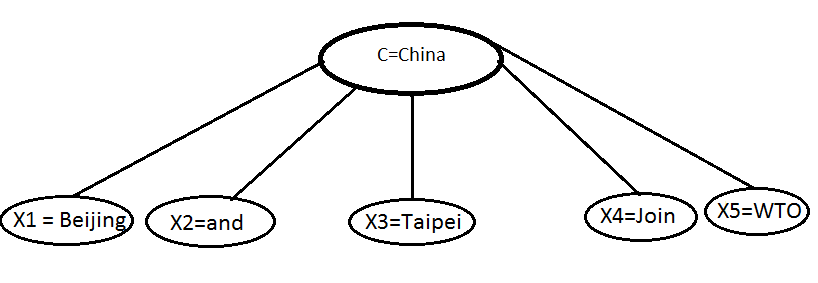
\includegraphics{MultiNomialNBModel}}
		\caption{Multinomial NB Model}
		\label{Multinomial NB Model}
	\end{figure}
\end{center}

\begin{center}
	\begin{figure}[H]
		\scalebox{0.4}[0.4]{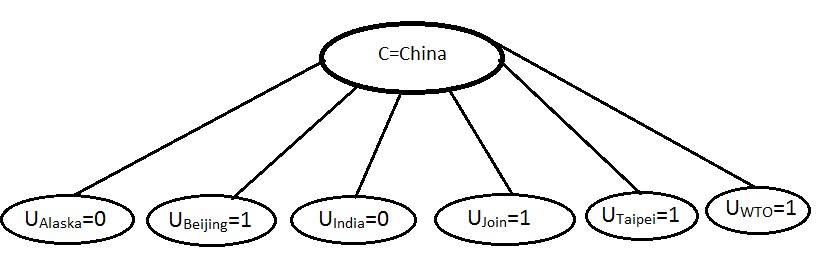
\includegraphics{BernoulliNBModel}}
		\caption{Bernoulli NB Model}
		\label{Bernoulli NB Model}
	\end{figure}\end{center}
We illustrate the conditional independence assumption in Figure \ref{Bernoulli NB Model} . The class China generates values for each of the five term attributes (multinomial) or six binary attributes (Bernoulli) with a certain probability, independent of the values of the other attributes. The fact that a document in the class China contains the term Taipei does not make it more likely or less likely that it also contains Beijing.
In reality, the conditional independence assumption does not hold for text data. Terms are conditionally dependent on each other. NB models perform well despite the conditional independence assumption. Even when assuming conditional independence, we still have too many parameters for the multinomial model if we assume a different probability distribution for each position in the document. The position of a term in a document by itself does not carry information about the class.
Although there is a difference between China sues France and France sues China, the occurrence of China in position 1 versus position 3 of the document is not useful in NB classification because we look at each term separately. The conditional independence assumption commits us to this way of processing the evidence. Also, if we assumed different term distributions for each position \textit{k}, we would have to estimate a different set of parameters for each \textit{k}. The probability of bean appearing as the first term of a coffee document could be different from it appearing as the second term, and so on. This again causes problems in estimation owing to data sparseness. For these reasons, we make a second independence assumption for the multinomial model, \textit{positional independence} : The conditional probabilities for a term are the same independent of position in the document.
\begin{equation}
	P(X_{k_{1}}=t|c)=P(X_{k_{2}}=t|c)
\end{equation}
for all positions \textit{k1,k2}, terms \textit{t} and classes \textit{c}. Thus, we have a single distribution of terms that is valid for all positions $k_{i}$ and we can use X as its symbol. Positional independence is equivalent to adopting the bag of words model.
With conditional and positional independence assumptions, we only need to estimate $\theta(M|C|)$ parameters $P(t_{k}|c)$(multinomial model) or $P(e_{i}|c)$(Bernoulli model), one for each term-class combination, rather than a number that is at least exponential in \textit{M}, the size of the vocabulary. The independence assumptions reduce the number of parameters to be estimated by several orders of magnitude.
To summarize, we generate a document in the multinomial model \ref{Multinomial NB Model} by first picking a class \textit{C=c} with \textit{P(c)} where \textit{C} is a random variable taking values from \textit{c} as values. Next we generate term \textit{$t_{k}$} in position \textit{k} with $P(X_{k}=t_{_{k}}|c)$ for each of the \textit{$ n_{d} $} positions of the document. The \textit{$X_{k}$} all have the same distribution over terms for a given \textit{c}. In the example in Figure \ref{Bernoulli NB Model} , we show the generation of $<t_{1},t_{2},t_{3},t_{4},t_{5}>=<Beijing,and,Taipei,join,WTO>$, corresponding to the one-sentence document Beijing and Taipei join WTO. 
For a completely specified document generation model, we would also have to define a distribution \textit{$P(n_{d}|c)$}
over lengths. Without it, the multinomial model is a token generation model rather than a document generation model. We generate a document in the Bernoulli model (Figure \ref{Bernoulli NB Model} ) by first picking a class \textit{C=c} with P(c) and then generating a binary indicator \textit{$e_{i}$} for each term \textit{$t_{i}$} of the vocabulary $(1\le i \le M)$. In the example in Figure \ref{Bernoulli NB Model} , we show the generation of , corresponding, again, to the one-sentence document Beijing and Taipei join WTO where we have assumed that `and' is a stop word.
\begin{table}[H]
	\caption{Multinomial vs Bernoulli Model}
		\label{Multinomial vs Bernoulli Model}
	\hspace{1pt}
	\setlength{\tabcolsep}{2pt}
	\renewcommand{\arraystretch}{2}
	\begin{tabular}{|p{2cm}|p{3cm}|p{3cm}|}
		\hline
		& \textbf{Multinomial model} & \textbf{Bernoulli model}\\
		\hline
		Event Model & generation of token & generation of document\\
		\hline
		Random Variable(s)& X = t iff t occurs at given pos & $U_{t}$ iff t occurs in doc\\
		\hline
		Document Representation & $d=<t_{1},...,t_{k},...t_{n_{d}}>,t_{k} \in V $& $d=<e_{1},...e_{i},..e_{M}>, e_{i} \in {0,1}$\\
		\hline
		Parameter estimation & P(X=t|c) & $P(U_{i}=e_{i}|c)$\\
		\hline
		Decision Rule:maximize& $P(c)\prod_{t_{i}\in V}P(U_i=e_i|c)$ & $P(c)\prod_{1\le k \le n_d}P(t_k|c)$\\
		\hline
		multiple occurrences & taken into account & ignored\\
		\hline
		length of docs & can handle longer docs & works best for short docs\\
		\hline
		\# features & can handle more & works best with fewer\\
		\hline
		estimate for term `the'& P(X=the|c)=0.05 & $P(U_{the}=1|c)=1.0$\\
		\hline
	\end{tabular}
\end{table}\vspace{-2pt}
We compare the two models in Table \ref{Multinomial vs Bernoulli Model}, including estimation equations and decision rules. Naive Bayes is so called because the independence assumptions we have just made are indeed very naive for a model of natural language. The conditional independence assumption states that features are independent of each other given the class. This is hardly ever true for terms in documents. In many cases, the opposite is true. In addition, the multinomial model makes an assumption of positional independence. The Bernoulli model ignores positions in documents altogether because it only cares about absence or presence. This \textit{bagofwords} model discards all information that is communicated by the order of words in natural language sentences. How can NB be a good text classifier when its model of natural language is so oversimplified?

\begin{table}[H]
	\caption{Correct estimation implies accurate prediction, but accurate prediction does not imply correct estimation }
	\label{Correct estimation implies accurate prediction, but accurate prediction does not imply correct estimation }
	\centering
	\setlength{\tabcolsep}{2pt}
	\renewcommand{\arraystretch}{3}
	\begin{tabular}{|c|p{2cm}|p{2cm}|p{1cm}|}
		\hline
		& \textbf{C1} & \textbf{C2} & \textbf{Class selected}\\
		\hline
		true probability P(c|d) & 0.6 & 0.4 & $c_1$ \\
		\hline
		$P(c)\prod_{1\le k \le n_d}P(t_k|c)$ & 0.00099 & 0.00001 & $c_1$\\
		\hline
		NB estimate P(c|d)& 0.99 & 0.01 & $c_1$\\ 
		\hline
	\end{tabular}
\end{table}

The answer is that even though the probability estimates of NB are of low quality, its classification decisions are surprisingly good. Consider a document \textit{d} with true probabilities $P(c_{1}|d)$=0.6 and $P(c_{2}|d)$=0.4 as shown in Table \ref{Correct estimation implies accurate prediction, but accurate prediction does not imply correct estimation } . Assume that d contains many terms that are positive indicators for \textit{c1} and many terms that are negative indicators for \textit{c2}. Thus, when using the multinomial model in Equation 13, $P(c_{1})\prod_{1\le k \le n_{d}}P(t_{k}|c1)$ will be much larger than $P(c_{2})\prod_{1\le k \le n_{d}}P(t_{k}|c2)$ (0.00099 vs. 0.00001 in the table). After division by 0.001 to get well-formed probabilities for $\textit{P(c|d)}$, we end up with one estimate that is close to 1.0 and one that is close to 0.0. This is common: The winning class in NB classification usually has a much larger probability than the other classes and the estimates diverge very significantly from the true probabilities. But the classification decision is based on which class gets the highest score. It does not matter how accurate the estimates are. Despite the bad estimates, NB estimates a higher probability for \textit{$c_{1}$}and therefore assigns to the correct class in Table \ref{Correct estimation implies accurate prediction, but accurate prediction does not imply correct estimation } . Correct estimation implies accurate prediction, but accurate prediction does not imply correct estimation. NB classifiers estimate badly, but often classify well. \newline
Even if it is not the method with the highest accuracy for text, NB has many virtues that make it a strong contender for text classification. It excels if there are many equally important features that jointly contribute to the classification decision. It is also somewhat robust to noise features and concept drift \textendash\hspace{0.04in} the gradual change over time of the concept underlying a class like US president from Bill Clinton to George W. Bush. Classifiers like kNN knn can be carefully tuned to idiosyncratic properties of a particular time period. This will then hurt them when documents in the following time period have slightly different properties.\newline
The Bernoulli model is particularly robust with respect to concept drift. The most important indicators for a class are less likely to change. Thus, a model that only relies on these features is more likely to maintain a certain level of accuracy in concept drift.
\subsection{Multinomial Model}
In contrast to the multi-variate Bernoulli event model,the multinomial model captures word frequency information in documents. Consider, for example, the occurrence of numbers in the Reuters newswire articles; our tokenization maps all strings of digits to a common token. Since every news article is dated, and thus has a number, the number token in the multi-variate Bernoulli event model is uninformative. However, news articles about earnings tend to have a lot of numbers compared to general news articles. Thus, capturing frequency information of this token can help classification.
In the multinomial model, a document is an ordered sequence of word events, drawn from the same vocabulary V . We assume that the lengths of documents are independent of class. We again make a similar naive Bayes assumption: that the probability of each word event in a document is independent of the word's context and position in the document. Thus, each document $d_i$ is drawn from a multinomial distribution of words with as many independent trials as the length of $d_{i}$. This yields the familiar 'bag of words' representation for documents. Define $N_{it}$ to be the count of the number of times word $w_t$ occurs in document $d_{i}$.
Then, the probability of a document given its class is simply the multinomial distribution:
\begin{equation}	
	P(d_{i}|c_{j};\theta)=P(|d_{i}|)|d_{i}|!\prod_{t=1}^{|V|}\frac{P(w_{t}|c_{j};\theta)^{N_{it}}}{N_{it!}}	
\end{equation}
The parameters of the generative component for each class are the probabilities for each word, written $\theta_{ w_{t} |c_{j}} = P(w_{t}|c_{j}; \theta)$, where $0 \le \theta w_{t} |c_{j} \le 1$ and $\sum_{t} \theta_{ w_{t} |c_{j} }= 1$.
Again, we can calculate Bayes-optimal estimates for these parameters from a set of labeled training data. Here, the estimate of the probability of word $w_{t}$ in class $c_{j}$ is:
\begin{equation}
	\theta_{w_{t}|c_{j}}=P(w_{t}|c_{j};\theta)=\frac{1+\sum_{i=1}^{|D|}N_{it}P(c_{j}|d_{i})}{|V|+\sum_{s=1}^{|V|}\sum_{i=1}^{|D|}N_{is}P(c_{j}|d_{i})}
\end{equation}
\subsection{Classifier Model}
There are two different ways we can set up an NB classifier. The model we introduced in the previous section is the multinomial model. It generates one term from the vocabulary in each position of the document, where we assume a generative model.
An alternative to the multinomial model is the multivariate Bernoulli model or Bernoulli model . It is equivalent to the binary independence model, which generates an indicator for each term of the vocabulary, either \textit{1} indicating presence of the term in the document or \textit{0} indicating absence. The Bernoulli model has the same time complexity as the multinomial model.
{
	\begin{algorithm}[H]
		\caption{Bernoulli Algorithm}
		\label{test}
		TrainBernoulliNB(C,D)
		\begin{algorithmic}[1]
			\STATE V $\leftarrow$ ExtractVocabulary(D) 
			\STATE N $\leftarrow$ CountDocs(D) 
			\FOR{each $c \in C $}
			\STATE\it $N_{c}$ $\leftarrow$ CountDocsInClass(D,c)
			\STATE \it $prior[c]$ $\leftarrow$ $N_{c}/N$
			\FOR {each $t \in V $}
			\STATE \it $N_{ct}$ $\leftarrow$ CountDocsInClassContainingTerm(D,c,t)
			\ENDFOR
			\ENDFOR
			\STATE \it $condprob[t][c]$ $\leftarrow$ $(N_{ct}+1)/(N_{c}+2)$
			\STATE return V, prior, condprob
		\end{algorithmic}		
		
		ApplyBernoulliNB(C,V,prior,condprob,d)
		\begin{algorithmic}[1]
			
			\STATE $V_{d}$ $\leftarrow$ ExtractTermsFromDoc(V,d) 
			\FOR{each $c \in C $}
			\STATE\it score[c] $\leftarrow$ log prior[c]
			\FOR {each $t \in V $}
			\IF {\it $t \in V_{d} $}
			\STATE \it score[c]+=log condprob[t][c]
			\ELSE
			\STATE \it score[c]+=log(1-condprob[t][c])
			\ENDIF
			\ENDFOR
			\ENDFOR
			\STATE return $argmax_{c \in C}score[c]$
		\end{algorithmic}
	\end{algorithm}
}
The different generation models imply different estimation strategies and different classification rules.
The Bernoulli model estimates P(t|c) as the fraction of documents of class that contain term. In contrast, the multinomial model estimates as the fraction of tokens or fraction of positions in documents of class \textit{c} that contain term \textit{t}. When classifying a test document, the Bernoulli model uses binary occurrence information, ignoring the number of occurrences, whereas the multinomial model keeps track of multiple occurrences. As a result, the Bernoulli model typically makes many mistakes when classifying long documents. For example, it may assign an entire book to the class China because of a single occurrence of the term China.
The models also differ in how non-occurring terms are used in classification. They do not affect the classification decision in the multinomial model, but in the Bernoulli model the probability of nonoccurrence is factored in when computing P(c|d).
This is because only the Bernoulli NB model models absence of terms explicitly.
\section{Proposed Algorithm}
\subsection{Block Diagram}
	\begin{center}
		\begin{figure}[H]
			\begin{mdframed}
			\scalebox{0.5}[0.5]{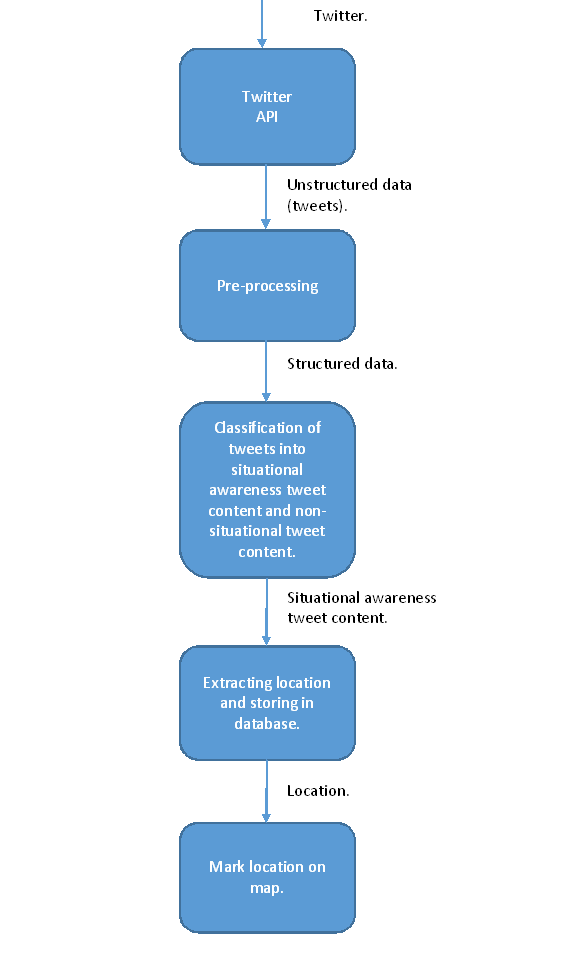
\includegraphics{BE-Block-Diagram}}
						\end{mdframed}
%			\caption{Block Diagram}
			\label{BlockDiagram}
		\end{figure}
	\end{center}
\begin{enumerate}
	\item[Step 1] Initially, Twitter data is streamed using Twitter APIs using the access keys and tokens which are needed for authentication. 
	\item[Step 2] Now this data is unstructured and needs to be preprocessed. Tweet preprocessing will be done by removing the stop-words(such as the, from, here, your), emoticons, URLs and unnecessary punctuation marks.
	\item[Step 3] The Bernoulli model,is a probabilistic model which,on the basis of training data, will classify the tweets into situational and non-situational.
	\item[Step 4] If the tweets are situational, we extract the co-ordinates from the Location Table and locations from the Tweet Table.
	\item[Step 5] We finally map the individual accident with Red markers and Accident Prone Areas using Blue Markers on Google Maps.
\end{enumerate}
\section{Output and Screenshots}
\begin{center}
	\begin{figure}[H]
		\scalebox{0.5}[0.5]{
\includegraphics{SituationalTweet}}
		\caption{Situational Tweet}
		\label{SituationalTweet}
	\end{figure}
\end{center}

\begin{center}
	\begin{figure}[H]
		\scalebox{0.5}[0.5]{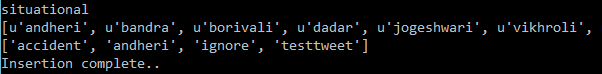
\includegraphics{Situational}}
		\caption{Classified : Situational}
		\label{ClassifiedSituational}
	\end{figure}
\end{center}

\begin{center}
	\begin{figure}[H]
		\scalebox{0.5}[0.5]{
\includegraphics{NonSituationalTweet}}
		\caption{Non Situational Tweet}
		\label{NonSituationalTweet}
	\end{figure}
\end{center}
\begin{center}
	\begin{figure}[H]
		\scalebox{0.5}[0.5]{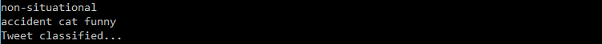
\includegraphics{NonSituational}}
		\caption{Classified : Non-Situational}
		\label{ClassifiedNonSituational}
	\end{figure}
\end{center}
\begin{center}
	\begin{figure}[H]
		\scalebox{0.5}[0.5]{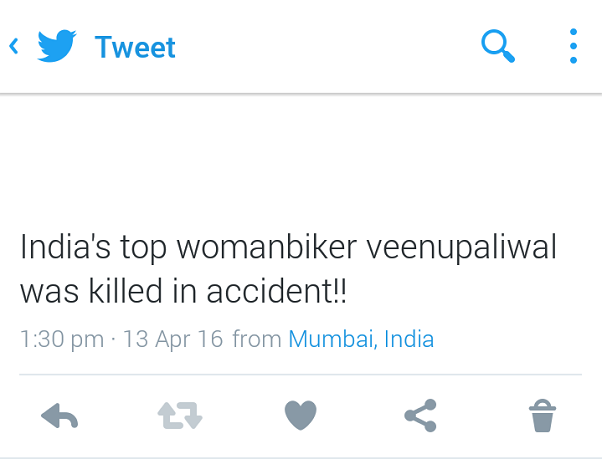
\includegraphics{FalsePositiveTweet}}
		\caption{An example of a False Positive Tweet}
		\label{FalsePositiveTweet}
	\end{figure}
\end{center}
\begin{center}
	\begin{figure}[H]
		\scalebox{0.5}[0.5]{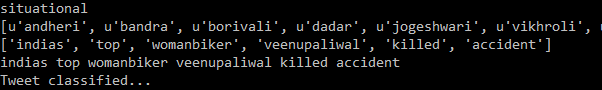
\includegraphics{FalsePositive}}
		\caption{An example of a False Positive(i.e.non-situational tweet classified as situational)}
		\label{FalsePositive}
	\end{figure}
\end{center}
\begin{center}
	\begin{figure}[H]
		\scalebox{0.5}[0.5]{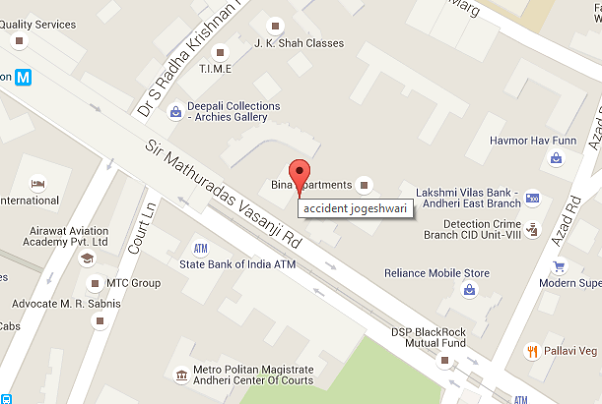
\includegraphics{IndividualAccident}}
		\caption{Individual Accident}
		\label{IndividualAccident}
	\end{figure}
\end{center}
\begin{center}
	\begin{figure}[H]
		\scalebox{0.5}[0.5]{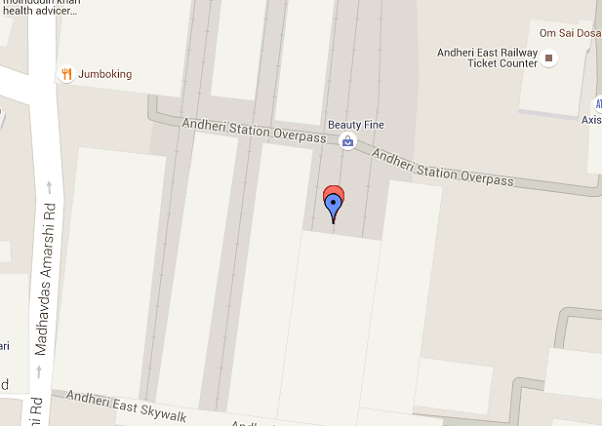
\includegraphics{AccidentProne}}
		\caption{Accident Prone Area}
		\label{AccidentProne}
	\end{figure}
\end{center}
\begin{center}
	\begin{figure}[H]
		\scalebox{0.5}[0.5]{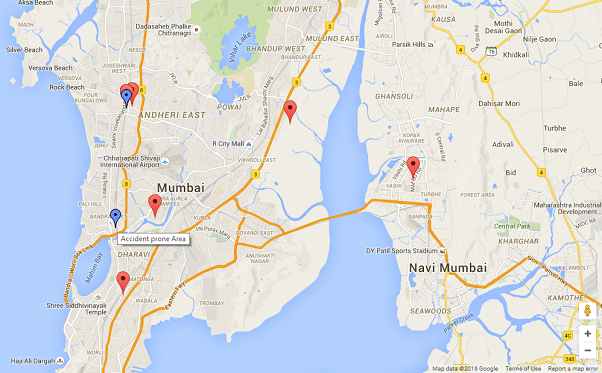
\includegraphics{FinalOutput}}
		\caption{Final Output}
		\label{FinalOutput}
	\end{figure}
\end{center}
\newpage
\section{Accuracy}
\begin{center}
	\begin{figure}[H]
		\scalebox{0.5}[0.5]{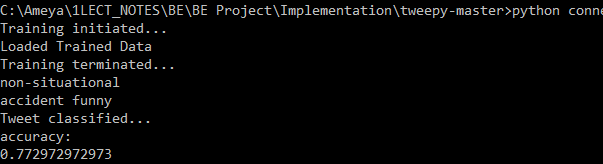
\includegraphics{accuracy}}
		\caption{Accuracy of classifier (for 182 test tweets)}
		\label{Accuracy}
	\end{figure}
\end{center}
\begin{table}[H]
	\caption{Accuracy Table}
	\label{Accuracy Table}
	\setlength{\tabcolsep}{3pt}
	\renewcommand{\arraystretch}{3}
	\begin{tabular}{|c|c|c|}
		\hline
		\textbf{No. of training tweets} & \textbf{No. of testing tweets} & \textbf{Accuracy}\\
		\hline
		200 & 182 & 77.29\% \\
		\hline
		%		$P(c)\prod_{1\le k \le n_d}P(t_k|c)$ & 0.00099 & 0.00001 \\
		%		\hline
		%		NB estimate P(c|d)& 0.99 & 0.01 \\ 
		%		\hline
	\end{tabular}
\end{table}
Accuracy is calculated using the formula:\vspace{0.5cm}\newline
Accuracy(in \%) \newline= $\dfrac{No.\ of\ correctly\ classified\ Tweets}{Total\ No.\ of\ Tweets} * 100$

\section{Conclusion}
We have learnt and implemented the following techniques: data streaming techniques, classification techniques and mapping techniques. For streaming the data in real-time from Twitter, we have written our code in python using the Tweepy framework. We have programmed the Bernoulli's model for classifying the tweets which contribute to situational awareness. Finally, we have implemented the Google Maps to map our results. We have trained the model using 100 situational tweets and 100 non-situational tweets. We have tested the model by sending real time tweets and recording the response. We have achieved the accuracy of 77.29\%.\newline
We hope to present this project as platform to keep a track on accident prone regions in Mumbai. The government agencies as well as several NGO's will now have a direct way to keep an eye on accident prone regions whereas the general public will know which route to avoid at a given time. Since the data is crowd-sourced, the entire responsibility of data is shared among users. We have implemented 2 levels of filters in order to root out the misleading tweets. However, the problem of false positives needs greater efforts and we hope to solve the same in future. The major benefits of this project include but not limited to: Low cost and crowd-sourced solution for a problem almost everyone faces in their lifetime, Saves human life and resources, Quick and real time response during times of emergency, No need of expensive hardware, sensors, trackers, cameras, etc.

% An example of a floating figure using the graphicx package.
% Note that \label must occur AFTER (or within) \caption.
% For figures, \caption should occur after the \includegraphics.
% Note that IEEEtran v1.7 and later has special internal code that
% is designed to preserve the operation of \label within \caption
% even when the captionsoff option is in effect. However, because
% of issues like this, it may be the safest practice to put all your
% \label just after \caption rather than within \caption{}.
%
% Reminder: the "draftcls" or "draftclsnofoot", not "draft", class
% option should be used if it is desired that the figures are to be
% displayed while in draft mode.
%
%\begin{figure}[!t]
%\centering
%\includegraphics[width=2.5in]{myfigure}
% where an .eps filename suffix will be assumed under latex, 
% and a .pdf suffix will be assumed for pdflatex; or what has been declared
% via \DeclareGraphicsExtensions.
%\caption{Simulation results for the network.}
%\label{fig_sim}
%\end{figure}

% Note that the IEEE typically puts floats only at the top, even when this
% results in a large percentage of a column being occupied by floats.


% An example of a double column floating figure using two subfigures.
% (The subfig.sty package must be loaded for this to work.)
% The subfigure \label commands are set within each subfloat command,
% and the \label for the overall figure must come after \caption.
% \hfil is used as a separator to get equal spacing.
% Watch out that the combined width of all the subfigures on a 
% line do not exceed the text width or a line break will occur.
%
%\begin{figure*}[!t]
%\centering
%\subfloat[Case I]{\includegraphics[width=2.5in]{box}%
%\label{fig_first_case}}
%\hfil
%\subfloat[Case II]{\includegraphics[width=2.5in]{box}%
%\label{fig_second_case}}
%\caption{Simulation results for the network.}
%\label{fig_sim}
%\end{figure*}
%
% Note that often IEEE papers with subfigures do not employ subfigure
% captions (using the optional argument to \subfloat[]), but instead will
% reference/describe all of them (a), (b), etc., within the main caption.
% Be aware that for subfig.sty to generate the (a), (b), etc., subfigure
% labels, the optional argument to \subfloat must be present. If a
% subcaption is not desired, just leave its contents blank,
% e.g., \subfloat[].


% An example of a floating table. Note that, for IEEE style tables, the
% \caption command should come BEFORE the table and, given that table
% captions serve much like titles, are usually capitalized except for words
% such as a, an, and, as, at, but, by, for, in, nor, of, on, or, the, to
% and up, which are usually not capitalized unless they are the first or
% last word of the caption. Table text will default to \footnotesize as
% the IEEE normally uses this smaller font for tables.
% The \label must come after \caption as always.
%
%\begin{table}[!t]
%% increase table row spacing, adjust to taste
%\renewcommand{\arraystretch}{1.3}
% if using array.sty, it might be a good idea to tweak the value of
% \extrarowheight as needed to properly center the text within the cells
%\caption{An Example of a Table}
%\label{table_example}
%\centering
%% Some packages, such as MDW tools, offer better commands for making tables
%% than the plain LaTeX2e tabular which is used here.
%\begin{tabular}{|c||c|}
%\hline
%One & Two\\
%\hline
%Three & Four\\
%\hline
%\end{tabular}
%\end{table}


% Note that the IEEE does not put floats in the very first column
% - or typically anywhere on the first page for that matter. Also,
% in-text middle ("here") positioning is typically not used, but it
% is allowed and encouraged for Computer Society conferences (but
% not Computer Society journals). Most IEEE journals/conferences use
% top floats exclusively. 
% Note that, LaTeX2e, unlike IEEE journals/conferences, places
% footnotes above bottom floats. This can be corrected via the
% \fnbelowfloat command of the stfloats package.

% if have a single appendix:
%\appendix[Proof of the Zonklar Equations]
% or
%\appendix  % for no appendix heading
% do not use \section anymore after \appendix, only \section*
% is possibly needed

% use appendices with more than one appendix
% then use \section to start each appendix
% you must declare a \section before using any
% \subsection or using \label (\appendices by itself
% starts a section numbered zero.)
%

%
%\appendices
%\section{Proof of the First Zonklar Equation}
%Appendix one text goes here.
%
%% you can choose not to have a title for an appendix
%% if you want by leaving the argument blank
%\section{}
%Appendix two text goes here.
%
%
%% use section* for acknowledgment
%\section*{Acknowledgment}
%
%
%The authors would like to thank...
%
%
%% Can use something like this to put references on a page
%% by themselves when using endfloat and the captionsoff option.
%\ifCLASSOPTIONcaptionsoff
%  \newpage
%\fi



% trigger a \newpage just before the given reference
% number - used to balance the columns on the last page
% adjust value as needed - may need to be readjusted if
% the document is modified later
%\IEEEtriggeratref{8}
% The "triggered" command can be changed if desired:
%\IEEEtriggercmd{\enlargethispage{-5in}}

% references section

% can use a bibliography generated by BibTeX as a .bbl file
% BibTeX documentation can be easily obtained at:
% http://mirror.ctan.org/biblio/bibtex/contrib/doc/
% The IEEEtran BibTeX style support page is at:
% http://www.michaelshell.org/tex/ieeetran/bibtex/
%\bibliographystyle{IEEEtran}
% argument is your BibTeX string definitions and bibliography database(s)
%\bibliography{IEEEabrv,../bib/paper}
%
% <OR> manually copy in the resultant .bbl file
% set second argument of \begin to the number of references
% (used to reserve space for the reference number labels box)
\bibliographystyle{IEEEtran}
\bibliography{project-ref}

% biography section
% 
% If you have an EPS/PDF photo (graphicx package needed) extra braces are
% needed around the contents of the optional argument to biography to prevent
% the LaTeX parser from getting confused when it sees the complicated
% \includegraphics command within an optional argument. (You could create
% your own custom macro containing the \includegraphics command to make things
% simpler here.)
%\begin{IEEEbiography}[{\includegraphics[width=1in,height=1.25in,clip,keepaspectratio]{mshell}}]{Michael Shell}
% or if you just want to reserve a space for a photo:

%\begin{IEEEbiography}{Michael Shell}
%Biography text here.
%\end{IEEEbiography}
%
%% if you will not have a photo at all:
%\begin{IEEEbiographynophoto}{John Doe}
%Biography text here.
%\end{IEEEbiographynophoto}
%
%% insert where needed to balance the two columns on the last page with
%% biographies
%%\newpage
%
%\begin{IEEEbiographynophoto}{Jane Doe}
%Biography text here.
%\end{IEEEbiographynophoto}

% You can push biographies down or up by placing
% a \vfill before or after them. The appropriate
% use of \vfill depends on what kind of text is
% on the last page and whether or not the columns
% are being equalized.

%\vfill

% Can be used to pull up biographies so that the bottom of the last one
% is flush with the other column.
%\enlargethispage{-5in}



% that's all folks
\end{document}


